\newpage
\section{Metodologia Experimental}

    \subsection{Materiais}
        O material utilizado para realização do experimento foi:

        \begin{itemize}
            \item U-2970A Gerador de dados;
            \item U-2970B Formatador de dados;
            \item U-2970C Modulador balanceado duplo;
            \item U-2970F Regenerador de clock de dados;
            \item U-2970G Recuperador de dados;
            \item U-2970H Receptor de dados;
            \item U-2970K Módulo de áudio;
            \item U-2970M Fonte de alimentação;
            \item U-2970N Conjunto de cabos de alimentação;
            \item 1 Gerador de função;
            \item 1 Osciloscópio de 2 canais.
        \end{itemize}

        Para execução do experimento, faz-se necessário executar os passos abaixo, de acordo com o roteiro disponibilizado em sala de aula.

    \subsection{Método para sinalização digital}
        \subsubsection{Estabelecendo a geração de dados}
            Conectar o módulo Gerador de dados U-2970A na fonte de alimentação U-2970M e verificar se a fonte de alimentação está ligada. Fazer as conexões e selecionar as duas chaves como mostra a figura \ref{fig:e1a}.
        
            \begin{figure}[H]
                \centering
                \caption{Sinais de Clock, Bit e Palavra.}
                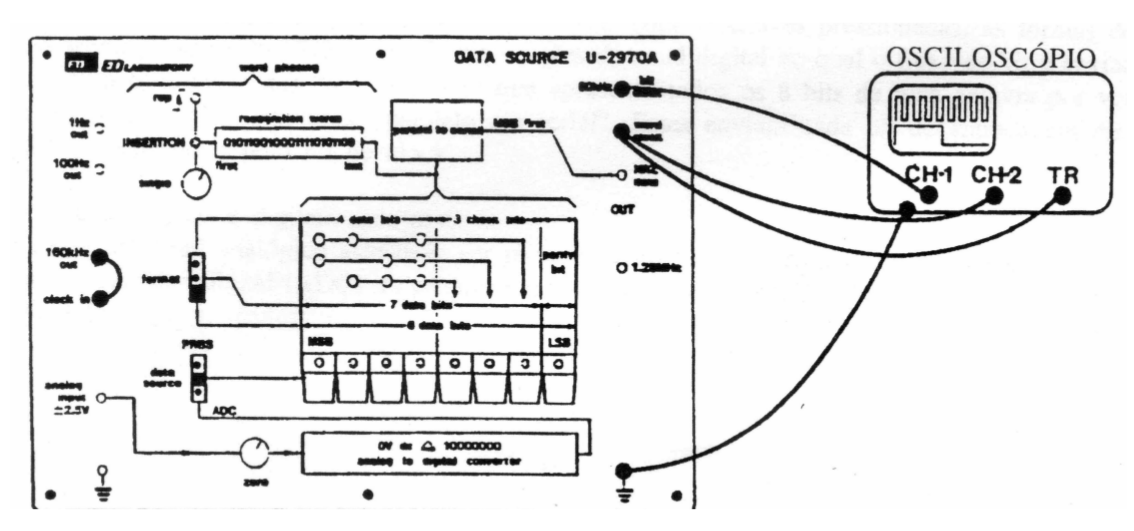
\includegraphics[scale=0.4]{e1a}
            
                \small Fonte: Jacob, J. L., Roteiro de laboratório, 2016.
                \label{fig:e1a}
            \end{figure}
        
        
        \subsubsection{Enviando um sinal analógico e digitalizando-o}
            \begin{figure}[H]
                \centering
                \caption{Entrada analógica para sistema digital.}
                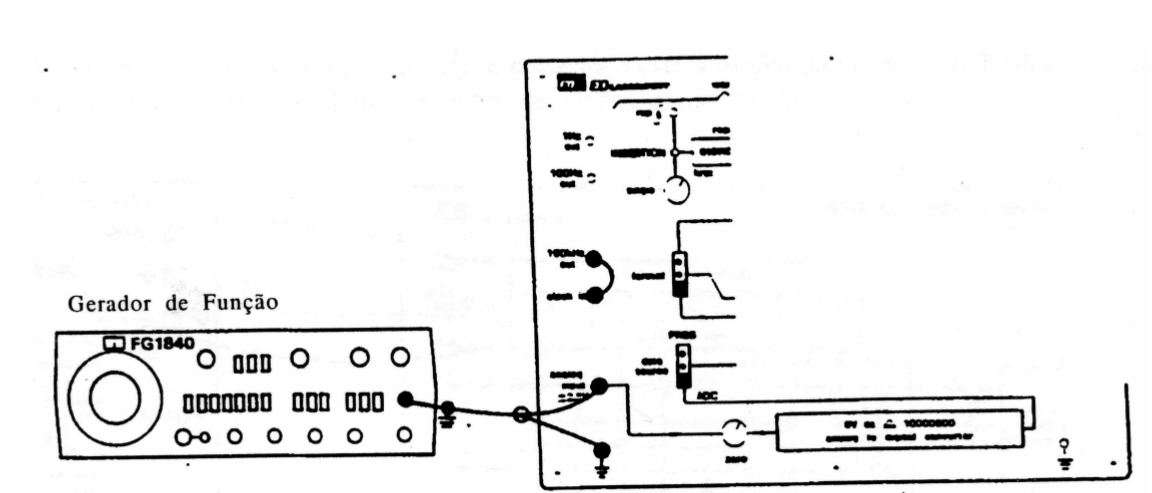
\includegraphics[scale=0.4]{e2a}
                
                \small Fonte: Jacob, J. L., Roteiro de laboratório, 2016.
                \label{fig:e2a}
            \end{figure}
            
            \begin{enumerate}
                \item Na sequência enviar um sinal analógico que deve ser primeiro convertido na forma digital. O gerador de dados tem um conversor analógico-digital (ADC) no próprio módulo. Selecione o ADC, usando a parte do canto esquerdo do módulo, figura \ref{fig:e2a}.
                
                \item Os bits do sinal não são agora determinados pelo push button e sim pela tensão no soquete de entrada analógica. Use o potenciômetro pequeno para ajustar a palavra de dados para 10000000.
                
                \item Agora conectar o gerador de função (figura 3) para fornecer um sinal analógico. Selecionar no gerador de função para o procedimento: onda triangular; 4 Vpp, 0,01Hz.
                
                \item Conectar o gerador de função para entrada analógica e terminal terra. A conduta da palavra de dados deve ser agora reconhecido como contador binário (ao contrário do final da rampa da entrada do triângulo). Isso devido a entrada do sinal analógico mudar, pois o ADC correspondente gera números binários. A saída de dados varia de acordo com a sinalização NRZ. A figura 4 mostra parte da sequência dos números binários.
            \end{enumerate}
    
        \subsubsection{Recebendo Palavras Códigos}
             \begin{figure}[H]
                 \centering
                 \caption{Receptor de dados.}
                 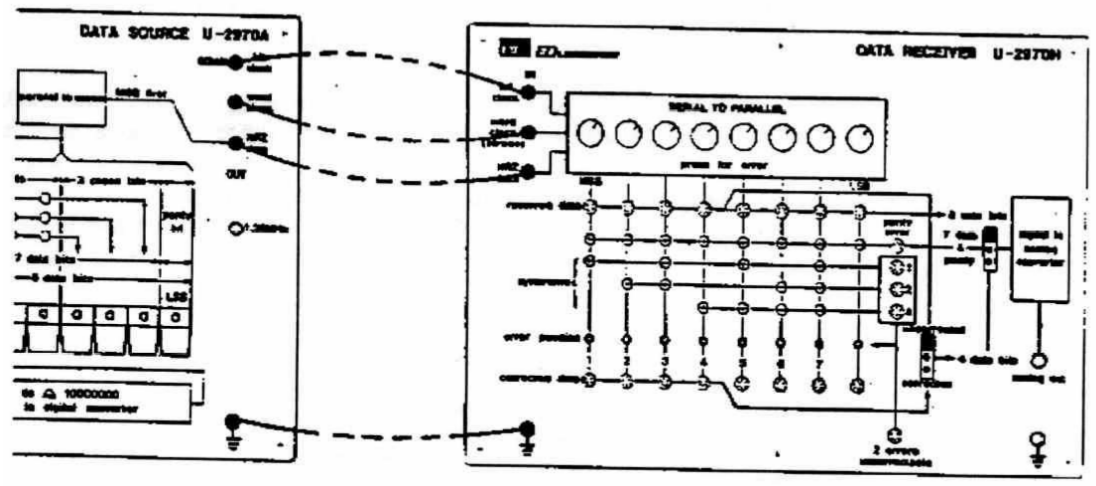
\includegraphics[scale=0.4]{e3a}
                        
                 \small Fonte: Jacob, J. L., Roteiro de laboratório, 2016.
                 \label{fig:e3a}
             \end{figure}
                    
            \begin{enumerate}
                \item Adicionar o módulo receptor de dados, U-2970H, e colocar este a direita do gerador de dados e conectar os dois juntos, selecionar as duas chaves no receptor de dados como na figura \ref{fig:e3a}.
                
                \item Se tudo estiver correto, a lâmpada de recepção do módulo receptor de dados deve agora mostrar o mesmo exemplo que nós estamos enviando a fonte. Mesmo alterando a frequência do sinal de entrada ele continua a ser aplicado. Tente aumentá-las (mas não aumente a tensão de entrada acima de 5 Vpp).
            \end{enumerate}
            
         \subsubsection{Obtendo Saída Analógica}
         
            \begin{enumerate}
                \item Se a saída for apresentada para um dispositivo analógico a palavra recebida é processada pelo conversor digital-analógico (DAC). O DAC é permanentemente conectado no módulo receptor U2970H.   
                
                \item Conectar o osciloscópio da seguinte maneira: CH1 na entrada analógica do gerador de dados; CH2 na saída analógica do receptor de dados; trigger no gerador de função (é ideal conectar na saída auxiliar TTL de onda quadrada).
                
                \item A base de tempo precisará ajustar para igualar a frequência do gerador de função. Se o anterior for de 100Hz, a base de tempo deve ser de 20ms por divisão para este instante.
                
                \item Nós agora temos um sistema simples de comunicação digital que aceitará um sinal de entrada analógico, convertendo-o para um fluxo de dígitos para transmissão, enviando para uma localidade remota e produzindo uma saída analógica que é uma cópia boa da entrada original. Nós podemos usá-la para enviar um sinal telefônico.
            \end{enumerate}
            
            \subsubsection{Operando o Módulo de Áudio U-2970K}
                \begin{enumerate}
                    \item O módulo de áudio U-2970K pode trabalhar com um microfone (recebendo som e enviando sinal elétrico) ou como auto-falante (recebendo um sinal elétrico e enviando o som).
                    
                    \item Conectar os terminais de entrada do módulo de áudio no gerador de função e selecionar a chave deste para o alto-falante (não esqueça de conectar a fonte de alimentação). Provavelmente o primeiro som você não ouvirá muito bem. Aumente a frequência do gerador de função para 600Hz e ajuste no módulo o controle de nível. O som agora deve ser ouvido claramente.
                \end{enumerate}
                
            \subsubsection{Completando o Canal Digital de Áudio}
                \begin{figure}[H]
                    \centering
                    \caption{Transmissão digital do sinal de áudio.}
                    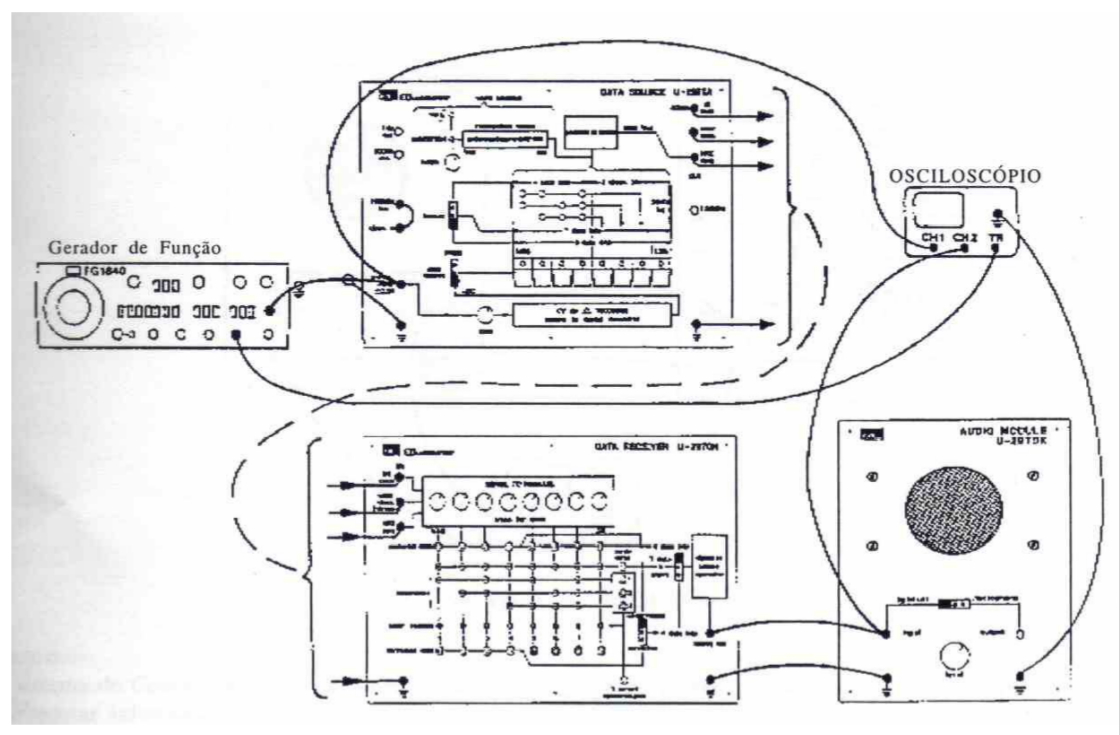
\includegraphics[scale=0.4]{e6a}
                                
                    \small Fonte: Jacob, J. L., Roteiro de laboratório, 2016.
                    \label{fig:e6a}
                \end{figure}
                \begin{enumerate}
                    \item O gerador de função está ligado no alto falante através de um par de fios cuja a função é de gravar nos terminais de entrada do alto-falante a tensão apresentada no terminal de saída do gerador. Mas esta função deve ser feita pelo sistema criado pelos módulos de dados e gerador de dados.
                    
                    \item Sem desfazer as conexões entre os módulos do gerador de dados e receptor de dados, desconecte a ligação entre o alto-falante e substitua a ligação de dados digitais como mostra a figura \ref{fig:e6a}. Se for feita corretamente, a conduta do alto-falante dever ser como a anterior.
                    
                    \item Isto mostra que o sinal de áudio pode ser enviado através dos módulos gerador de dados e receptor de dados. Mas por que a contradição, você pode perguntar, quando o mesmo par de fios fará o mesmo? Esta pergunta será discutida no próximo experimento.
                    
                    \item Tentar tirar do canal digital som e aumentar a frequência da forma de onda do sinal recebido.
                    Este será encontrado com uma frequência acima de 5kHz (metade da frequência do clock da palavra).
                    
                    \item Estas frequências não são diretas devido ao sistema ser digital, mas é adequada para o sinal analógico que é uma amostra do clock da palavra padrão.
                \end{enumerate}
                
            \subsubsection{Testando um Telefone Simples}
                \begin{figure}[H]
                    \centering
                    \caption{Telefone digital simples.}
                    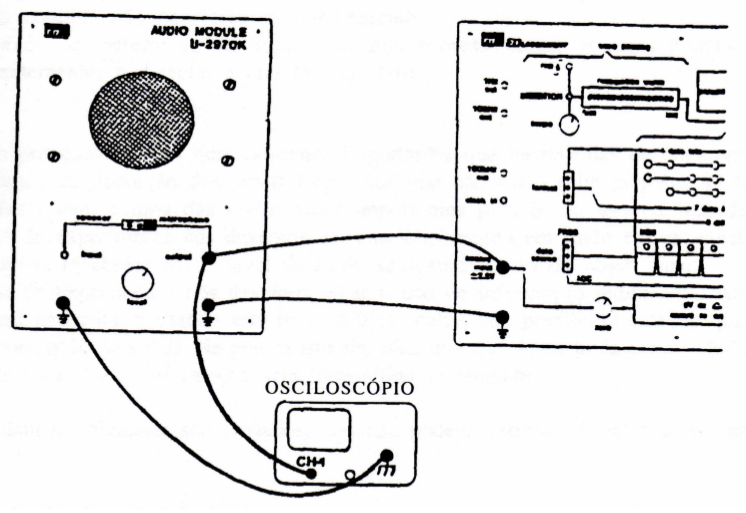
\includegraphics[scale=0.4]{e7a}
                    
                    \small Fonte: Jacob, J. L., Roteiro de laboratório, 2016.
                    \label{fig:e7a}
                \end{figure}
                
                \begin{enumerate}
                    \item Se o segundo módulo de áudio estiver disponível, este pode ser usado como microfone e troca-se o gerador de função, como na figura 7, com isso cria-se um telefone de uma via.
                    
                    \item Selecionar o osciloscópio da seguinte maneira: sensibilidade CH1 0.2V/divisão; base de tempo 1ms/divisão, livre funcionamento.
                    
                    \item Se o controle de nível do lado esquerdo do microfone é sintonizado no sentido horário, o osciloscópio deve mostrar agora o sinal de resposta para entrar algum ruído no módulo.
                    
                    \item Se resultar algum som de ruído, selecione o controle de nível para o lado direito do módulo do alto-falante (sentido anti-horário) até o som parar. Se você então ouvir fechado o alto falante deve ser habilitado para ouvir algum som entrando no microfone.rio, o osciloscópio deve mostrar agora o sinal de resposta para entrar algum ruído no módulo.
                    
                    \item A razão para estar ”chiando” é que o som que vem do alto falante alcança o microfone, que é
                    enviado novamente ao alto-falante formando um ciclo repetitivo. Se os módulos amplificam o suficiente igualando o som desprezando cada vez que for muito maior voltando para o ciclo. 
                    
                    Para verificar que isso não tem nada a ver com o sistema digital, troque-o conectando os fios diretamente entre os módulos de áudio.
                \end{enumerate}
                
        \subsection{Ruído}
            \subsubsection{Rejeição do seu próprio ruído}
            Fazer as conexões e selecionar o conjunto de chaves do módulo como mostra a figura 8. Os dois pinos do dispositivo de entrada dos dados quadrados no módulo U-2970F ambos são resistores de 2 $k\Omega$. Eles servem para atenuar o sinal e permitir um sinal de ruído para misturar com este.
            
            Observação: Salvar todas as curvas obtidos no osciloscópio e tirar uma foto a cada montagem. Usar esses dados no relatório.
            
                \begin{enumerate}
                    \item Inicialmente, selecionar a tensão de saída do gerador de função para zero;
                    
                    \item Configurar a palavra de dados no módulo gerador de dados (DATA SOURCE). A palavra 01001100 deve ser usada.
                    
                    \item O menor controle de polarização do módulo U-2970F deve ser ajustado para o meio da faixa em que o módulo receptor de dados (DATA RECEIVER) reproduzirá corretamente os dados originais da fonte.
                    
                    \item Nós agora temos um sinal uniforme (a palavra de dados configurada na fonte) sendo enviada para o receptor de dados que passa da forma analógica para o módulo de áudio. De forma semelhante, se o controle de nível no módulo de áudio é girado totalmente no sentido horário, o som não deve aparecer no módulo. Mas o que acontece se nós misturarmos alguns ruídos com o fluxo de bits de dados?
                    
                    \item Selecionar o gerador de função para a onda senoidal de 100 Hz. Incrementar a saída gradualmente, olhe no osciloscópio e ouça. Nada irá acontecer até um certo nível de ruído audível, a forma de onda do CH2 do osciloscópio ficará distorcida e as lâmpadas de dados recebidos, todas irão aparecer juntas.
                    
                    \item Ajustar a polarização dos dados enquadrados para cortar o ruído, então incrementar uma quantidade de ruído e o reajuste do maior nível possível atinge uma altura que o sistema não poderá responder.
                    
                    \item Com ambos os canais conectados na saída dos dados enquadrados, ajuste o osciloscópio até que os dois traços fiquem superpostos. Então reconecte como mostra a figura \ref{fig:e1b}. Desenhe a forma de onda. Tente alterar a quantidade de ruído e de polarização.
                    
                    \item Agora deve estar claro que a polarização tem de ser colocada, portanto o sinal de entrada barulhento não deve cruzar o valor de polarização exceto quando o valor do bit mudar. Fornecer isto faz com que a saída enquadrada não seja afetada pelo ruído e portanto, os dados são recebidos.
                \end{enumerate}
            
                \newpage
                \begin{figure}[H]
                    \centering
                    \caption{Simulação de ruído com um gerador de função.}
                    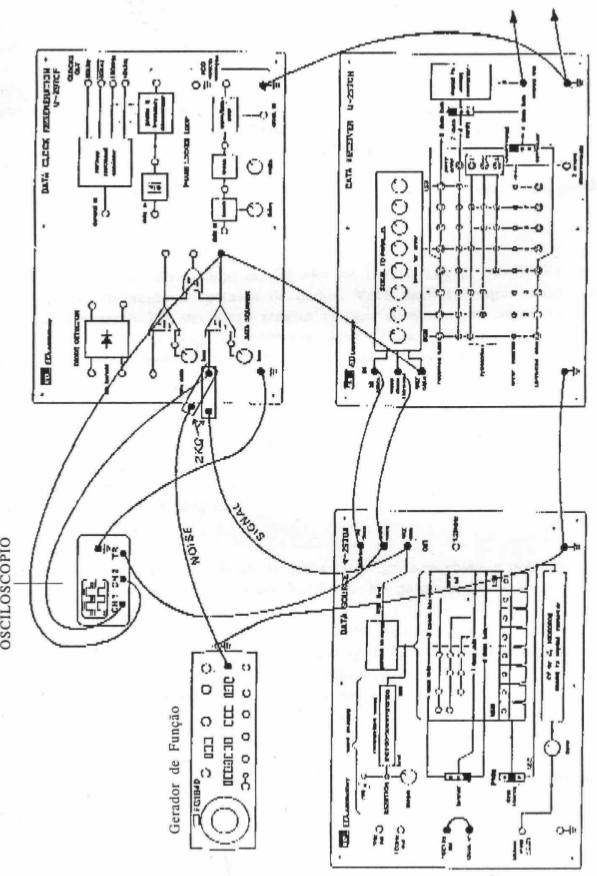
\includegraphics[scale=0.8]{e1b}
                    
                    \small Fonte: Jacob, J. L., Roteiro de laboratório, 2016.
                    \label{fig:e1b}
                \end{figure}
            
        \subsection{Detecção e correção de erros}
                        A forma mais simples de detectar o erro é verificar a paridade. Isto significa que a verificação é sempre número par (ou algumas vezes ímpar) de bits na palavra de dados. O código tem que ser disposto da mesma maneira que em um bit, chamado de bit de paridade e sempre ajustado para criar a correção do bit de paridade no gerador de dados. Portanto, se os 8 bits da palavra são usados, 7 bits podem levar os dados, enquanto o oitavo bit simplesmente completa a correção de paridade.
                        
                        A ideia é de que se uns dos bits for interrompido (mude para um estado oposto), a paridade virá errada. Este pode ser detectado no receptor e identifica-se que temos algum erro.
            Se mais de um bit esta corrompido não é mais possível identificar que bit está em erro, com isso
            este bit não pode ser corrigido.
            Se mais de dois bits estão com erro, estes criam um código que correspondem a alguns dados
            falsos, com ou sem o bit individual.
            
            \subsubsection{Verificando a Paridade}
                \begin{enumerate}
                    \item Selecionar a chave FORMAT do módulo de gerador de dados (DATA SOURCE) para a posição central. Tente produzir uma seleção diferente da palavra de dados . Você deve encontrar o bit a direita, este não pode ser selecionado individualmente. Em vez disso sempre vá para o estado que cria o número de bits ímpar (o bit de paridade é mostrado através da lâmpada verde para lembrar você de que este não é o bit de dados).
                    
                    \item Selecionar a chave a direita no módulo receptor de dados para a posição central dado ''7'' e um bit de paridade. A paridade será mostrada também no LED verde.
                    
                    \item O erro selecionado pode ser simulado em algum dos 8 bits recebidos pressionando as teclas pretas do módulo receptor de dados. Note que se alguns dos bits for modificado, este é mostrado no LED amarelo ''erro de paridade''. No entanto se o número de bits errado é par, detecta-se que não há erro de paridade. Desta maneira o receptor não pode dizer que o bit está com um erro. Para criar um erro mais evidente, chaveie os dados da fonte para o formato de 8 bits e a palavra de dados enviada tem um número impar de bits com erro para que o receptor mostre que o bit está com erro.
                \end{enumerate}
                
                
            \subsubsection{Correção do erro}
                \begin{enumerate}
                    \item A correção pode ser muito útil quando a palavra de dados corrompida recebida é colocada
                    a direita. Portanto, você vai descobrir uma forma simples de usar a verificação do bit de
                    paridade e também identificar um erro presente em qualquer parte da palavra.
                    
                    \item Para habilitar a correção de erros, o receptor precisa de mais informações. Diferentes bits
                    da palavra de dados devem ser usados com ”verificador de bits”e a checagem deve ser mais
                    complicada. Temos muitos códigos de ”correções de erros”, incluindo a família conhecida
                    como código Hamming. O ED-2970 utiliza o código relacionado nesta família de códigos.
                    
                    \item Selecionar a chave FORMAT do módulo gerador de dados (DATA SOURCE) para a posição
                    superior. Pressionar a tecla a esquerda (MSB) e mantenha pressionada. Depois de um
                    segundo, o display mostrará 4 bits acendendo os LEDs vermelhos e 4 bits acendendo os
                    LEDs verdes. Os LEDs verdes não são (antes como bit de paridade) indicadores do controle
                    direto, mas são selecionados automaticamente a medida que os 4 bits de dados vermelhos
                    são mudados.
                    
                    \item O bit menos significativo (LSB) é normal ser o bit de paridade, determinado por todos os
                    bits de dados. Cada nova checagem de bits é formada de acordo com a seleção da paridade
                    do grupo de bits de dados, como indicado no diagrama de módulo.
                    
                    \item Para ver se esta checagem extra de bits são usadas, selecionar a chave a direita no módulo
                    receptor para a posição 4 bits de dados.
                    
                    \item O conjunto vertical de 4 LEDs vermelhos (incluindo o indicador de erro de paridade) mostra
                    o resultado de 4 cheques de paridade em grupos diferentes de bits recebidos, como mostra o
                    diagrama no painel. A tecla das duas fileiras de LEDs mostra: posição do erro, detecta no
                    circuito o bit com erro; bits de dados correto, depois da correção através do circuito.
                    
                    \item Se não houver erro, nenhum dos 4 LEDs de paridade irão acender, os bits não foram corrigidos
                    e a fila de teclas de LEDs igualam-se ao do gerador de dados (DATA SOURCE).
                    
                    \item Agora pressionar uma das teclas de erro. Um ou mais LEDs de paridade devem acender.
                    Dependendo do bit de correção de erro, o circuito deve identificar o bit em que ocorreu o
                    erro e mostra o LED da coluna correspondente a posição do erro. Ao mesmo tempo o bit
                    correspondente será corrigido (isto é, igualando-se ao gerador de dados). Tente isto com cada
                    tecla de erro (uma de cada vez).
                    
                    \item A saída do conversor digital-analógico é chaveado através da chave interna de duas posições, o
                    receptor pode recebe dados corretos ou incorretos. Selecionar o gerador de função para enviar
                    um sinal de áudio através da entrada analógica do módulo de gerador de dados; enviar dados
                    corretos do módulo receptor de dados (RECEIVER MODULE) para o módulo de Áudio
                    (AUDIO MODULE); observar que o erro de um bit (individual) não afeta na recepção do
                    sinal. Compare com o resultado usando dados incorretos.
                \end{enumerate}

                
        \subsection{Método para regeneração do clock}
            \begin{enumerate}
                \item Configurar o equipamento como mostrado na figura 9, incluindo as 5 chaves. A saída final,
                ligações 23 e 24, podem ser conectadas para o módulo de áudio (configurado como um
                speaker).
                
                \item Configurar o osciloscópio: CH1 e CH2: acoplamento DC, 5V/divisão; base de tempo:
                10$\mu s$/divisão, trigado externamente por +VE indo para borda do clock da palavra.
                
                \item Conectar CH1 para a saída NRZ do módulo formato de dados U-2970B (observe que isto é
                atrasado de metade do tempo de bit comparado com a entrada NRZ). Conecte CH2 na saída
                bi-fásica, ligação 7.
                
                \item Configure vários padrões de bit e observe como o código bi-fase é relacionado aos dados
                básicos. Note que o sinal bi-fase corresponde aos dados na primeira metade de cada período
                de bit (isto é, antes da transição do sinal; na segunda metade tem-se a reversão).
                
                \item O que se pretende, portanto, é uma forma de tornar negativo (trocar a polaridade) do sinal
                durante a segunda metade do tempo de bit. Isto é feito com um clock funcionando a 80kHz
                e usando sua saída (ligação 12) para negar o sinal em meios ciclos alternados. A negação é
                realizada pelo modulador. Tal clock precisa ser sincronizado com os dados de chegada.
                
                \item Na prática um enlace de comunicação pode ser interposto entre uma extremidade e a outra
                das ligações 7 e 8. Um dado quadrado é usado para garantir transições precisas na ligação
                11.
                
                \item Transferir o osciloscópio CH para a ligação 11 e o soquete para a sua direita. Note que
                a forma de onda gera, pela unidade d/dt, um pequeno pulso em cada transição do sinal
                quadrado. Então um pulso de sincronização é gerado no centro de todos os períodos de bit,
                mas somente algumas vezes entre os períodos de bit.
            \end{enumerate}
            
            \newpage
            \begin{figure}[H]
                \centering
                \caption{Regeneração do Clock e Recuperação dos Dados Bi-fase.}
                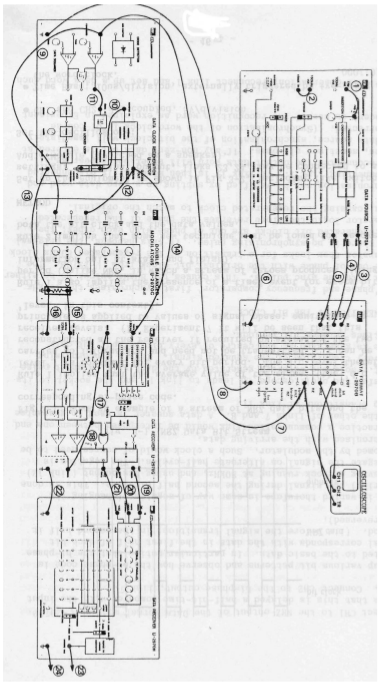
\includegraphics[scale=0.8]{e1d}
                
                \small Fonte: Jacob, J. L., Roteiro de laboratório, 2016.
                \label{fig:e1d}
            \end{figure}
            
        \subsection{Recuperação do bit de clock}
            O comparador de frequência e fase primeiro sincroniza os 160kHz de clock com os pulsos sync.
            Isto faz com que a saída de 80kHz seja dentro ou fora de fase com o clock do bit original de
            U-2970B. O comparador busca uma transição do clock regenerado de 80kHz quando não existe
            pulso de sincronismo. Se isso acontece, os clocks de bits originais e os regenerados estão fora de
            fase entre si; o comparador lógico por consequência reverte a fase do clock regenerador causando
            a regeneração do clock correspondente ao original.
            
            \begin{enumerate}
                \item A sincronização pode ser verificada pela configuração de uma palavra de dados zero e desco-
                nectando a ligação 1.
                \item Se a ligação 11 é então momentaneamente desconectada e reconectada, a palavra de dados
                de saída as vezes aparecerá como tudo zero e as vezes tudo um.
                \item Se algum bit de dados não zero sair da fonte de dados, a sincronização do bit de clock será
                imediatamente corrigida.
                \item Depois desta observação, reconecte a ligação 1 e configure a palavra de dados como 01011000.
            \end{enumerate}
            
            
        \subsection{Recuperação dos dados - INTEGRATE-AND-DUMP}
            \begin{enumerate}
                \item Mover o osciloscópio CH1 para a ligação 15. A forma de onda aqui é basicamente uma réplica
                dos dados originais na forma NRZ, mas com grandes picos sobrepostos. A técnica integrate-
                and-dump é útil para a recuperação de dados limpos de ondas com picos. O princípio é
                ilustrado na figura 11.
                \item. Conectar CH2 na saída do integrador em uso. Se o controle de polarização é um conjunto
                apropriado, a saída será vista aumentar em taxa que é positiva durante um bit 0 e negativa
                (isto é, queda) durante um bit 1. Em ambos os casos o integrador é zerado no fim do tempo
                de bit, pronto para reiniciar no próximo bit (uma sensibilidade de 2V/divisão pode tornar a
                exibição mais clara).
                \item É importante notar que alguns picos de duração curta, tal como aquelas em CH1, tem pouco
                efeito no nível do sinal em CH2.
                \item O sinal de saída do integrador poderia ser suficiente para representar os dados, mesmo se o
                sinal transportar ruído de pico para além dos picos de amplitude fixos existentes.
                \item Os dados recuperados podem ser vistos movendo-se o CH1 para a ligação 17.
            \end{enumerate}
            
            
         